% Created 2025-03-28 Fri 10:44
% Intended LaTeX compiler: pdflatex
\documentclass[bigger]{beamer}
\usepackage[utf8]{inputenc}
\usepackage[T1]{fontenc}
\usepackage{graphicx}
\usepackage{grffile}
\usepackage{longtable}
\usepackage{wrapfig}
\usepackage{rotating}
\usepackage[normalem]{ulem}
\usepackage{amsmath}
\usepackage{textcomp}
\usepackage{amssymb}
\usepackage{capt-of}
\usepackage{hyperref}
\usepackage[spanish, mexico, english]{babel}
\uselanguage{Spanish}
\languagepath{Spanish}
\usepackage{mathtools}
%%%%%%%%%%%%%%%%%%%%%%%%%%%%%%%%%%%%%%%%%%%%%%%%%%%%%%%%%%%%%%%%%%%%%%%%%%%%%%%%%%%%%%%%
%% TEX code to draw an external link symbol                                           %%
%% See https://tex.stackexchange.com/questions/99316/symbol-for-external-links/294990 %%
%%%%%%%%%%%%%%%%%%%%%%%%%%%%%%%%%%%%%%%%%%%%%%%%%%%%%%%%%%%%%%%%%%%%%%%%%%%%%%%%%%%%%%%%

\usepackage{tikz}

\newcommand{\ExternalLink}{%
    \tikz[x=1.2ex, y=1.2ex, baseline=-0.05ex]{% 
        \begin{scope}[x=1ex, y=1ex]
            \clip (-0.1,-0.1) 
                --++ (-0, 1.2) 
                --++ (0.6, 0) 
                --++ (0, -0.6) 
                --++ (0.6, 0) 
                --++ (0, -1);
            \path[draw, 
                line width = 0.5, 
                rounded corners=0.5] 
                (0,0) rectangle (1,1);
        \end{scope}
        \path[draw, line width = 0.5] (0.5, 0.5) 
            -- (1, 1);
        \path[draw, line width = 0.5] (0.6, 1) 
            -- (1, 1) -- (1, 0.6);
    }
}


\usepackage{transparent}
\usetheme{Pittsburgh}
\usecolortheme{dove}
\author{Eric Magar}
\date{28-3-2025 \newline Univ. of Houston}
\title{Data in memory of Francisco Cantú}
\setbeamertemplate{footline}[frame number]{}
\setbeamertemplate{navigation symbols}{}
\expandafter\def\expandafter\insertshorttitle\expandafter{%
\insertshorttitle\hfill%
\insertframenumber}
%  \insertframenumber\,/\,\inserttotalframenumber}
\hypersetup{
 pdfauthor={Eric Magar},
 pdftitle={Data in memory of Francisco Cantú},
 pdfkeywords={},
 pdfsubject={},
 pdfcreator={Emacs 27.1 (Org mode 9.3)}, 
 pdflang={English}}
\begin{document}

\maketitle
\begin{frame}{Outline}
\tableofcontents
\end{frame}

\setbeamercovered{transparent}

\section{The colleague}
\label{sec:org0416fa5}
\begin{frame}[label={sec:org48900d3}]{Team player}
\begin{columns}
\begin{column}{0.5\columnwidth}
\begin{scriptsize}
\begin{itemize}
  \item Susan Achury
  \item Leonardo Antenangeli
  \item Natalia Aruguete
  \item Ernesto Calvo
  \item Scott Clifford
  \item Scott Desposato (x2)
  \item Cengiz Erisen
  \item Jorge Fernandes
  \item Omar García Ponce
  \item Agustina Haime
  \item Victor Hernández Huerta
  \item Verónica Hoyo (x2)
  \item Paul Johnson
  \item Sandra Ley (x2)
\end{itemize}
\end{footnotesize}
\end{column}
\begin{column}{0.5\columnwidth}
\begin{scriptsize}
\begin{itemize}
  \item Eric Magar
  \item Marco Morales
  \item Javier Márquez
  \item Margarita Ramírez
  \item Pedro Riera (x3) 
  \item Sebastián Saiegh
  \item Carlos Scartascini
  \item Leslie Schwindt-Bayer
  \item Robert Stein et al. (x2)
  \item Michelle Torres
  \item Agustín Vallejo
  \item Tiago Ventura
  \item Dane Wendell
  \item ...
\end{itemize}
\end{footnotesize}
\end{column}
\end{columns}
\end{frame}
\begin{frame}[label={sec:org5b3a55d}]{Three strands}
\begin{block}{Fraud, election integrity}
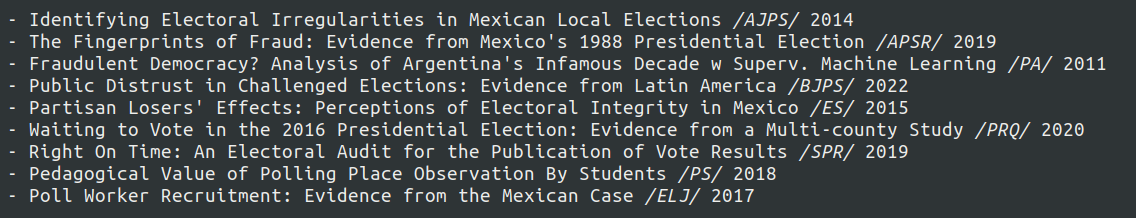
\includegraphics[width=\textwidth]{./pics/pubs1.png}
\end{block}
\begin{block}{Voting, vote trading}
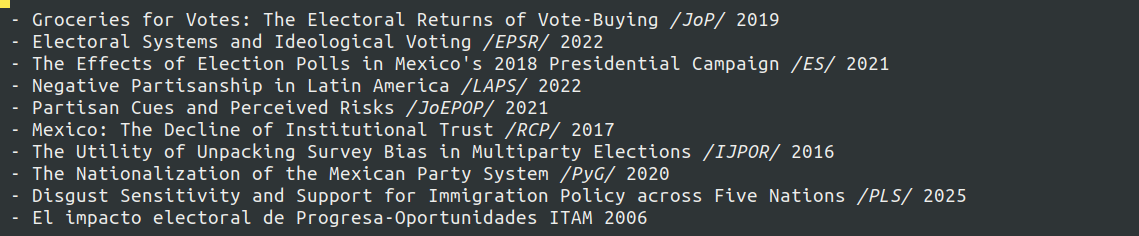
\includegraphics[width=\textwidth]{./pics/pubs2.png}
\end{block}
\begin{block}{Legislative studies, roll call votes}
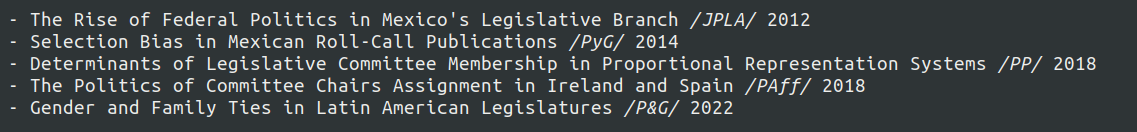
\includegraphics[width=\textwidth]{./pics/pubs3.png}
\end{block}
\end{frame}
\begin{frame}[label={sec:org43ab3ad}]{Three strands}
\begin{block}{Fraud, election integrity}
\transparent{0.3}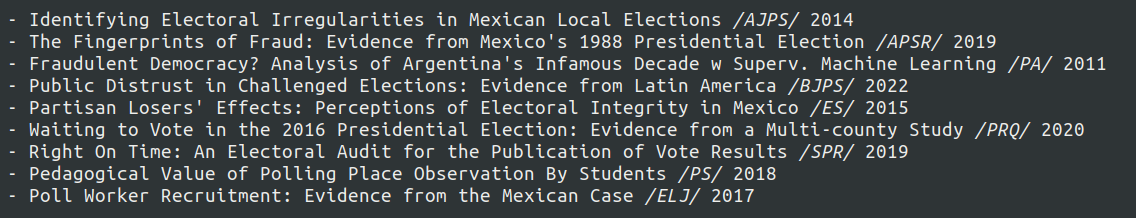
\includegraphics[width=\textwidth]{./pics/pubs1.png}
\end{block}
\begin{block}{Voting, vote trading}
\transparent{0.3}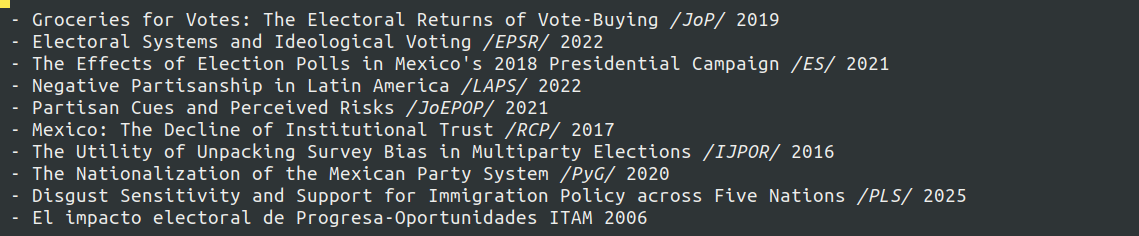
\includegraphics[width=\textwidth]{./pics/pubs2.png}
\end{block}
\begin{block}{Legislative studies, roll call votes}

\includegraphics[width=\textwidth]{./pics/pubs3s.png}
\end{block}
\end{frame}
\section{Senate roll call votes}
\label{sec:org739a45b}
\begin{frame}[label={sec:orgc12f6fd}]{In the back burner since 2014}
\begin{itemize}
\item Asymmetric approach to Mexican Congress \newline \(\rightarrow\) Francisco sought to remedy
\item But: Senate doesn't publish pre-digested roll call votes
\item Sent me a collection scraped from Senate web page \pause
\end{itemize}
\begin{block}{Labor intensive}
\begin{itemize}
\item Messy web concièrges
\item Agreed we'd deal with this later
\end{itemize}
\end{block}
\end{frame}
\begin{frame}[label={sec:orge1d857f}]{Problems}
\begin{block}{Unsystematic}
\begin{itemize}
\item In period covered, roll call vote appear in 3 dift ways
\item Member names often scrambled
\item Many repeats  \pause
\end{itemize}
\end{block}
\begin{block}{What I've done (just a start)}
\begin{enumerate}
\item \emph{Beautiful soup} to de-HTMLize
\item Full senator names, with substitutes
\item Coded regular expressions in search of patterns
\item Trial-and-error
\end{enumerate}
\end{block}
\end{frame}
\begin{frame}[label={sec:org4899f8f}]{What surfaced}
\begin{itemize}
\item Francisco sent 637 digital issues of \emph{Diario de sesiones}
\item Each records debate, floor proceedings, and 1+ roll call vote   \pause
\item Produced 724 votes in the dataset
\end{itemize}
\begin{center}
\begin{tabular}{rr}
Session & N\\
\hline
Spr. '05 & 101\\
Fall '05 & 118\\
Spr. '06 & 154\\
Fall '06 & 47\\
Spr. '07 & 104\\
Fall '07 & 17\\
Fall '10 & 73\\
Spr. '11 & 110\\
\end{tabular}
\end{center}
\end{frame}
\begin{frame}[label={sec:org894e77b}]{Against bill universe}
\begin{center}
\begin{tabular}{lrrr}
Session & Cantú & Weldon & dif\\
\hline
\alert{59th Leg.} &  &  & \\
Fall'03 &  & 109 & \\
Spr.'04 &  & 64 & \\
Fall'04 &  & 98 & \\
Spr.'05 & 101 & 108 & --7\\
Fall'05 & 118 & 130 & --12\\
Spr.'06 & 154 & 157 & --3\\
\hline
\alert{60th Leg.} &  &  & \\
Fall'06 & 47 & 63 & --16\\
Spr.'07 & 104 & 108 & --4\\
Fall'07 & 17 & 177 & --160\\
Spr.'08 &  & 109 & \\
Fall'08 &  & 132 & \\
Spr.'09 &  & 129 & \\
\end{tabular}
\end{center}
\end{frame}
\begin{frame}[label={sec:org1faaed2}]{Rice cohesion scores}
\centering
\(C_{pv} = \frac{\left|\text{ayes}_{pv} - \text{nays}_{pv}\right|}{\text{ayes}_{pv} + \text{nays}_{pv}}\)
\bigskip
\begin{center}
\begin{tabular}{lrr}
 & \(\bar{C}\) & \\
Party & 2005--06 & 2006--11\\
\hline
PAN & .96 & .98\\
PRI & .98 & .99\\
Left & .96 & .92\\
\end{tabular}
\end{center}
\end{frame}
\begin{frame}[label={sec:orga06c044}]{Rice dissimilarity}
\centering
\(D_{pqv} = \left|\frac{\text{nays}_{pv}}{\text{ayes}_{pv} + \text{nays}_{pv}} - \frac{\text{nays}_{qv}}{\text{ayes}_{qv} + \text{nays}_{qv}}\right|\)

\bigskip
\begin{center}
\begin{tabular}{crr}
 & \(\bar{D}\) & \\
 & 2005--06 & 2006--11\\
\hline
PAN--PRI & .07 & \alert{.06}\\
PAN--Left & .10 & \alert{.21}\\
PRI--Left & .07 & \alert{.18}\\
 &  & \\
\end{tabular}
\end{center}
\end{frame}
\section{Public repository}
\label{sec:orge5c57de}
\begin{frame}[label={sec:org7eb58e3},fragile]{Public repository}
 \url{https://github.com/emagar/senmex}
\bigskip \pause
\begin{block}{Files:}
\begin{columns}
\begin{column}{0.5\columnwidth}
\begin{itemize}
\item \texttt{votdat58.59.csv} (\(V\))
\item \texttt{sendat58.59.csv} (\(S\))
\item \texttt{rc58.59.csv}  (\(V \times S\))
\end{itemize}
\end{column}
\begin{column}{0.5\columnwidth}
\begin{itemize}
\item \texttt{votdat60.61.csv}
\item \texttt{sendat60.61.csv}
\item \texttt{rc60.61.csv} \pause \bigskip
\end{itemize}
\end{column}
\end{columns}
\end{block}
\begin{block}{More work needed\ldots{} crowdsourcing?}
\begin{itemize}
\item Missing votes in period
\item Extend coverage 1997--2025
\item Scale senator's ideal points
\end{itemize}
\end{block}
\end{frame}
\begin{frame}[label={sec:orgff1b844}]{.}
\centering 
Thank you \alert{Francisco}!
\end{frame}
\end{document}
